\chapter{Konveksitet}

\section{Konvekse Mengder}

\subsection{Definisjon}
\begin{definition}{Konveks Mengde}{convex_set}
    En mengde $C \subset \mathbb{R}^n$ er \textbf{konveks} hvis, for ethvert par punkter $x, y \in C$, ligger hele linjesegmentet som forbinder dem i $C$. Formelt:
    \[
    x, y \in C \quad \Longrightarrow \quad \alpha x + (1-\alpha) y \in C \quad \text{for alle}~\alpha \in [0, 1].
    \]
    Ekvivalent kan man si at enhver konveks kombinasjon av punkter i $C$ forblir i $C$.
\end{definition}

\begin{figure}[htb]
    \centering
    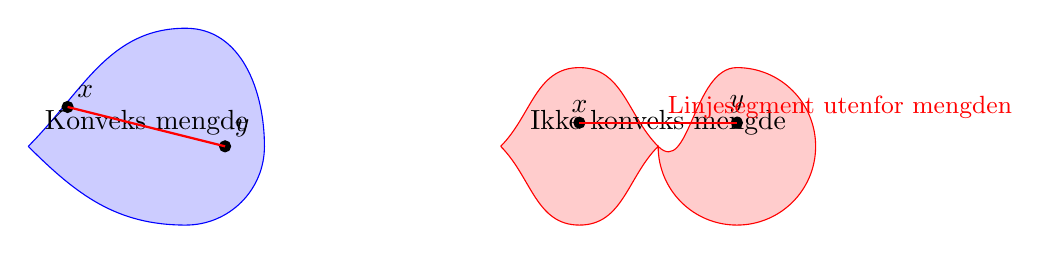
\begin{tikzpicture}
        % Convex set
        \draw[fill=blue!20, draw=blue] (0,0) to[out=45, in=180] (2,1.5) to[out=0, in=90] (3,0) to[out=270, in=0] (2,-1) to[out=180, in=315] (0,0);
        \node at (1.5, 0.3) {Konveks mengde};
        \filldraw[black] (0.5,0.5) circle (2pt) node[above right] {$x$};
        \filldraw[black] (2.5,0) circle (2pt) node[above right] {$y$};
        \draw[thick, red] (0.5,0.5) -- (2.5,0);
        
        % Non-convex set
        \begin{scope}[xshift=6cm]
            \draw[fill=red!20, draw=red] (0,0) to[out=45, in=180] (1,1) to[out=0, in=135] (2,0) to[out=315, in=180] (3,1) to[out=0, in=90] (4,0) to[out=270, in=0] (3,-1) to[out=180, in=270] (2,0) to[out=225, in=0] (1,-1) to[out=180, in=315] (0,0);
            \node at (2, 0.3) {Ikke-konveks mengde};
            \filldraw[black] (1,0.3) circle (2pt) node[above] {$x$};
            \filldraw[black] (3,0.3) circle (2pt) node[above] {$y$};
            \draw[thick, red] (1,0.3) -- (3,0.3);
            \node[red, right] at (2,0.5) {\small Linjesegment utenfor mengden};
        \end{scope}
    \end{tikzpicture}
    \caption{Illustrasjon av konvekse og ikke-konvekse mengder}
    \label{fig:convex_sets}
\end{figure}


\subsection{Eksempler}
\begin{example}{Vanlige Konvekse Mengder}{common_convex_sets}
    \begin{itemize}
        \item \textbf{Euklidske Kuler}: $\bigl\{ x : \|x - x_0\|\le r \bigr\}$ er konvekse fordi linjesegmenter mellom to punkter i en kule forblir inni.
        \item \textbf{Polyedre}: $\{x : A x \le b\}$ (ulikheter forstått komponentvis) er konvekse. Polytoper og simplekser er spesielle eksempler.
        \item \textbf{Affine Underrom}: $\{x : A x = b\}$ er konvekse.
        \item \textbf{Halvrom}: $\{x \in \mathbb{R}^n : a^T x \leq b\}$ er konvekse.
        \item \textbf{Kjegler}: $\{tx : t \geq 0, x \in C\}$ der $C$ er konveks er konvekse.
    \end{itemize}
\end{example}

\subsection{Operasjoner som Bevarer Konveksitet}
\begin{theorem}{Konveksitetsbevarende Operasjoner}{convexity_preserving}
    Følgende operasjoner bevarer konveksitet av mengder:
    \begin{itemize}
        \item \textbf{Snitt}: Snittet av enhver samling konvekse mengder er konveks.
        \item \textbf{Lineære eller Affine Avbildninger}: Hvis $T$ er en lineær (eller affin) transformasjon, og $C$ er konveks, er $T(C)$ konveks.
        \item \textbf{Minkowski Sum}: For konvekse $C_1,C_2$, er Minkowski-summen $\{x_1 + x_2 : x_1\in C_1, x_2\in C_2\}$ konveks.
        \item \textbf{Skalering og Translasjon}: For enhver $\alpha \in \mathbb{R}$ og $b \in \mathbb{R}^n$, er både $\alpha C$ og $C + b$ konvekse.
    \end{itemize}
\end{theorem}

\subsection{Ekstremalpunkter, Flater og Separasjon}
\begin{definition}{Ekstremalpunkt}{extreme_point}
    Et \textbf{ekstremalpunkt} i en konveks mengde $C$ er et punkt som ikke ligger i noe åpent linjesegment inneholdt i $C$ (bortsett fra det trivielle segmentet som starter og slutter i punktet selv).
\end{definition}

\begin{theorem}{Separasjonsteoremet}{separation_theorem}
    La $C$ og $D$ være disjunkte ikke-tomme konvekse mengder i $\mathbb{R}^n$.
    \begin{enumerate}
        \item Hvis $C$ er åpen, eksisterer det en ikke-null $p \in \mathbb{R}^n$ og $\alpha \in \mathbb{R}$ slik at $p^T x < \alpha \leq p^T y$ for alle $x \in C$ og $y \in D$.
        \item Hvis $C$ og $D$ er lukket og minst én er kompakt, eksisterer det en ikke-null $p \in \mathbb{R}^n$ og $\alpha, \beta \in \mathbb{R}$ slik at $p^T x \leq \alpha < \beta \leq p^T y$ for alle $x \in C$ og $y \in D$.
    \end{enumerate}
\end{theorem}

\begin{figure}[htb]
    \centering
    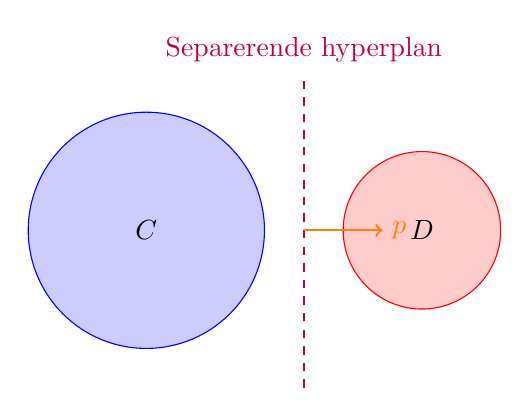
\begin{tikzpicture}
        % Første mengde (konveks)
        \draw[fill=blue!20, draw=blue] (0,0) circle (1.5);
        \node at (0, 0) {$C$};
        
        % Andre mengde (konveks)
        \draw[fill=red!20, draw=red] (3.5,0) circle (1);
        \node at (3.5, 0) {$D$};
        
        % Separerende hyperplan
        \draw[thick, dashed, purple] (2,-2) -- (2,2);
        \node[purple] at (2, 2.3) {Separerende hyperplan};
        
        % Normalvektor til hyperplanet
        \draw[->, thick, orange] (2,0) -- (3,0);
        \node[orange, right] at (3, 0) {$p$};
    \end{tikzpicture}
    \caption{Separasjon av to konvekse mengder med et hyperplan}
    \label{fig:separation}
\end{figure}

\section{Konvekse Funksjoner}

\subsection{Definisjon}
\begin{definition}{Konveks Funksjon}{convex_function}
    En funksjon $f: C \to \mathbb{R}$, med $C \subset \mathbb{R}^n$ konveks, er \textbf{konveks} hvis
    \[
    f\bigl(\alpha x + (1-\alpha) y \bigr) \;\le\; \alpha\, f(x) \;+\;(1-\alpha)\, f(y)\quad \text{for alle }x,y \in C,\;\alpha \in [0, 1].
    \]
    Intuitivt ligger grafen til $f$ "under korden" som forbinder to punkter på grafen.
\end{definition}

\begin{figure}[htb]
  \centering
  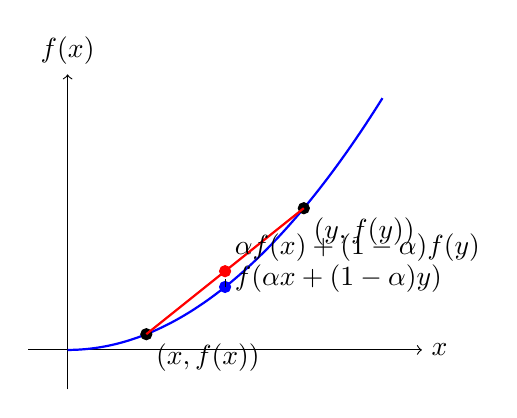
\begin{tikzpicture}
    % Axes
    \draw[->] (-0.5,0) -- (4.5,0) node[right] {$x$};
    \draw[->] (0,-0.5) -- (0,3.5) node[above] {$f(x)$};
    
    % Convex function (parabola)
    \draw[thick, blue] plot [domain=0:4, samples=100] (\x, {0.2*\x*\x});
    
    % Points on the function
    \filldraw[black] (1,0.2) circle (2pt) node[below right] {$(x,f(x))$};
    \filldraw[black] (3,1.8) circle (2pt) node[below right] {$(y,f(y))$};
    
    % Chord
    \draw[red, thick] (1,0.2) -- (3,1.8);
    
    % Midpoint on chord
    \filldraw[red] (2,1) circle (2pt);
    
    % Point on function at same x
    \filldraw[blue] (2,0.8) circle (2pt);
    
    % Vertical line connecting points
    \draw[dashed] (2,0.8) -- (2,1);
    
    % Labels
    \node[right] at (2,0.9) {$f(\alpha x + (1-\alpha)y)$};
    \node[above right] at (2,1) {$\alpha f(x) + (1-\alpha)f(y)$};
  \end{tikzpicture}
  \caption{En konveks funksjon ligger under korden som forbinder to punkter på dens graf}
  \label{fig:convex_function}
\end{figure}

\subsection{Ekvivalente Karakteriseringer}
\begin{theorem}{Karakteriseringer av Konveksitet}{convexity_characterizations}
  For en funksjon $f: C \to \mathbb{R}$ på et konvekst domene $C$:
  \begin{itemize}
    \item \textbf{Førsteordens Betingelse} (når $f$ er deriverbar):
    \[
    f(y)\;\ge\; f(x) + \nabla f(x)^\mathsf{T}\,(y - x), \quad \text{for alle }x, y \in C.
    \]
    Med ord: den lineære approksimasjonen (tangenten) ved $x$ er en global undereestimator av $f$.
    
    \item \textbf{Andreordens Betingelse} (når $f$ er to ganger deriverbar):
    \[
    \nabla^2 f(x)\; \text{er positiv semidefinitt for alle }x \in C.
    \]
    Det vil si at Hessian-matrisen er positiv semidefinitt overalt i $C$.
  \end{itemize}
\end{theorem}

\begin{figure}[htb]
  \centering
  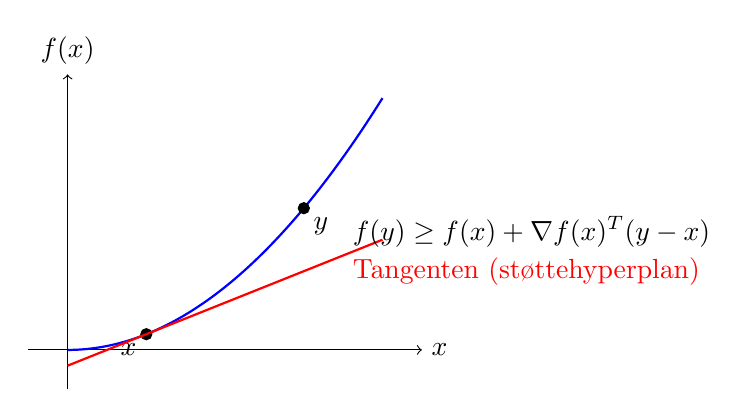
\begin{tikzpicture}
    % Axes
    \draw[->] (-0.5,0) -- (4.5,0) node[right] {$x$};
    \draw[->] (0,-0.5) -- (0,3.5) node[above] {$f(x)$};
    
    % Convex function (parabola)
    \draw[thick, blue] plot [domain=0:4, samples=100] (\x, {0.2*\x*\x});
    
    % Point on the function
    \filldraw[black] (1,0.2) circle (2pt) node[below left] {$x$};
    \filldraw[black] (3,1.8) circle (2pt) node[below right] {$y$};
    
    % Tangent at x
    \draw[red, thick] plot [domain=0:4, samples=100] (\x, {0.2*1*1 + 0.4*1*(\x-1)});
    
    % Labels
    \node[right] at (3.5,1.5) {$f(y) \geq f(x) + \nabla f(x)^T(y-x)$};
    \node[red, right] at (3.5,1) {Tangenten (støttehyperplan)};
  \end{tikzpicture}
  \caption{Førsteordens karakterisering av konveksitet: funksjonen ligger over sine tangentplan}
  \label{fig:first_order}
\end{figure}

\subsection{Eksempler}
\begin{example}{Vanlige Konvekse Funksjoner}{common_convex_functions}
  \begin{itemize}
    \item \textbf{Lineære eller Affine Funksjoner}: $f(x) = c^\mathsf{T} x + \beta$ er konvekse (og også konkave).
    \item \textbf{Normer}: $f(x) = \|x\|_p$ for $p \geq 1$ er konvekse.
    \item \textbf{Kvadratiske Former}: $f(x) = x^\mathsf{T} Q x$ er konveks hvis og bare hvis $Q$ er positiv semidefinitt.
    \item \textbf{Eksponential}: $f(x) = e^{\alpha x}$ (i én dimensjon) eller $f(x)= \exp(\langle \alpha, x \rangle)$ (multidimensjonal) er konveks.
    \item \textbf{Logaritmisk Barriere}: $f(x) = -\log(x)$ på $\mathbb{R}_{++}$ er konveks.
    \item \textbf{Entropi}: $f(x) = x\log(x)$ på $\mathbb{R}_{++}$ er konveks.
  \end{itemize}
\end{example}

\begin{table}[htb]
  \centering
  \begin{tabular}{|l|l|c|}
    \hline
    \textbf{Funksjon} & \textbf{Domene} & \textbf{Konveksitet} \\
    \hline
    $f(x) = c^Tx + b$ & $\mathbb{R}^n$ & Konveks og konkav \\
    $f(x) = \|x\|_p$, $p \geq 1$ & $\mathbb{R}^n$ & Konveks \\
    $f(x) = x^TQx$, $Q \succeq 0$ & $\mathbb{R}^n$ & Konveks \\
    $f(x) = e^x$ & $\mathbb{R}$ & Konveks \\
    $f(x) = -\log(x)$ & $\mathbb{R}_{++}$ & Konveks \\
    $f(x) = x\log(x)$ & $\mathbb{R}_{++}$ & Konveks \\
    $f(x) = 1/x$ & $\mathbb{R}_{++}$ & Konveks \\
    $f(x) = \max\{x_1, x_2, \ldots, x_n\}$ & $\mathbb{R}^n$ & Konveks \\
    \hline
  \end{tabular}
  \caption{Eksempler på vanlige konvekse funksjoner}
  \label{tab:convex_functions}
\end{table}

\subsection{Vanlige Egenskaper}
\begin{theorem}{Operasjoner som Bevarer Funksjonskonveksitet}{function_convexity_preserving}
  Følgende operasjoner bevarer funksjonskonveksitet:
  \begin{itemize}
    \item \textbf{Ikke-negative Vektede Summer}: Hvis $f_1, f_2, \ldots, f_n$ er konvekse og $\alpha_1, \alpha_2, \ldots, \alpha_n \geq 0$, da er $\sum_{i=1}^n \alpha_i f_i$ konveks.
    
    \item \textbf{Punktvis Maksimum}: Hvis $f_1, f_2, \ldots, f_n$ er konvekse, da er $\max\{f_1, f_2, \ldots, f_n\}$ konveks.
    
    \item \textbf{Punktvis Supremum}: Hvis $f_\alpha$ er konveks for hver $\alpha \in A$, da er $\sup_{\alpha \in A} f_\alpha$ konveks.
    
    \item \textbf{Sammensetning med Affin Funksjon}: Hvis $f$ er konveks og $A$ er en matrise og $b$ er en vektor, da er $g(x) = f(Ax + b)$ konveks.
    
    \item \textbf{Minimering over Noen Variabler}: Hvis $f(x,y)$ er felles konveks i $(x,y)$, da er $g(x) = \inf_y f(x,y)$ konveks i $x$.
  \end{itemize}
\end{theorem}

\subsection{Subgradienter (Generelle Derivater)}
\begin{definition}{Subgradient}{subgradient}
  For en konveks funksjon $f: C \to \mathbb{R}$, er en vektor $g \in \mathbb{R}^n$ en \textbf{subgradient} av $f$ ved $x \in C$ hvis
  \[
  f(y)\;\ge\; f(x)\;+\; g^\mathsf{T}\,(y-x),\quad \forall y \in C.
  \]
  Mengden av alle subgradienter av $f$ ved $x$ kalles \textbf{subdifferensialet} av $f$ ved $x$, og betegnes med $\partial f(x)$.
\end{definition}

\begin{figure}[htb]
  \centering
  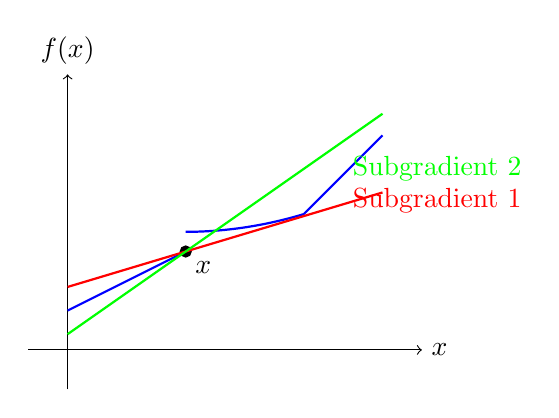
\begin{tikzpicture}
    % Axes
    \draw[->] (-0.5,0) -- (4.5,0) node[right] {$x$};
    \draw[->] (0,-0.5) -- (0,3.5) node[above] {$f(x)$};
    
    % Convex function (piecewise)
    \draw[thick, blue] plot [domain=0:1.5, samples=50] (\x, {0.5*\x + 0.5});
    \draw[thick, blue] plot [domain=1.5:3, samples=50] (\x, {1.5 + 0.1*(\x-1.5)^2});
    \draw[thick, blue] plot [domain=3:4, samples=50] (\x, {1.5 + 0.1*(3-1.5)^2 + 1*(\x-3)});
    
    % Point of non-differentiability
    \filldraw[black] (1.5,1.25) circle (2pt) node[below right] {$x$};
    
    % Subgradients
    \draw[red, thick] plot [domain=0:4, samples=50] (\x, {1.25 + 0.3*(\x-1.5)});
    \draw[green, thick] plot [domain=0:4, samples=50] (\x, {1.25 + 0.7*(\x-1.5)});
    
    % Labels
    \node[red, right] at (3.5,1.9) {Subgradient 1};
    \node[green, right] at (3.5,2.3) {Subgradient 2};
  \end{tikzpicture}
  \caption{Subgradienter av en konveks funksjon ved et punkt der den ikke er deriverbar}
  \label{fig:subgradients}
\end{figure}

\section{Grunnleggende Resultater og Implikasjoner}

\subsection{Jensens Ulikhet}
\begin{theorem}{Jensens Ulikhet}{jensens_inequality}
  For enhver konveks funksjon $f: C \to \mathbb{R}$ og punkter $x_1, x_2, \ldots, x_k \in C$:
  \[
  f\Bigl(\sum_{i=1}^k \alpha_i x_i \Bigr) \;\le\; \sum_{i=1}^k \alpha_i\, f(x_i),
  \]
  når $\alpha_i\ge 0$ og $\sum_{i=1}^k \alpha_i=1$.
  
  For stokastiske variabler, hvis $X$ er en stokastisk variabel med verdier i $C$ og $f$ er konveks, da:
  \[
  f(\mathbb{E}[X]) \leq \mathbb{E}[f(X)]
  \]
  forutsatt at forventningsverdiene eksisterer.
\end{theorem}

\subsection{Konveks Programmering}
\begin{definition}{Konvekst Optimeringsproblem}{convex_optimization_problem}
  Et konvekst optimeringsproblem har formen:
  \begin{mini*}
    {x \in \mathbb{R}^n}{f(x)}{}{}
    \addConstraint{g_i(x) \leq 0,}{i = 1, \ldots, m}
    \addConstraint{h_j(x) = 0,}{j = 1, \ldots, p}
  \end{mini*}
    
  hvor $f$ og $g_i$ er konvekse funksjoner, og $h_j(x) = a_j^Tx - b_j$ er affine funksjoner.
\end{definition}

\begin{theorem}{Egenskaper ved Konveks Optimering}{convex_optimization_properties}
  For et konvekst optimeringsproblem:
  \begin{enumerate}
    \item Enhver lokal minimerer er en global minimerer.
    \item Mengden av minimerere, hvis ikke-tom, er konveks.
    \item Hvis $f$ er strengt konveks, har problemet høyst én løsning.
    \item KKT-betingelsene er nødvendige og tilstrekkelige for optimalitet (under kvalifikasjonsbetingelser).
  \end{enumerate}
\end{theorem}

\subsection{Epigraf-Formulering}
\begin{definition}{Epigraf}{epigraph}
  \textbf{Epigrafen} til en funksjon $f: C \to \mathbb{R}$ er mengden
  \[
  \mathrm{epi}(f) \;=\; \{(x,t)\mid x\in C,\; t\ge f(x)\}.
  \]
  En funksjon $f$ er konveks hvis og bare hvis $\mathrm{epi}(f)$ er en konveks mengde i $\mathbb{R}^{n+1}$.
\end{definition}

\begin{figure}[htb]
  \centering
  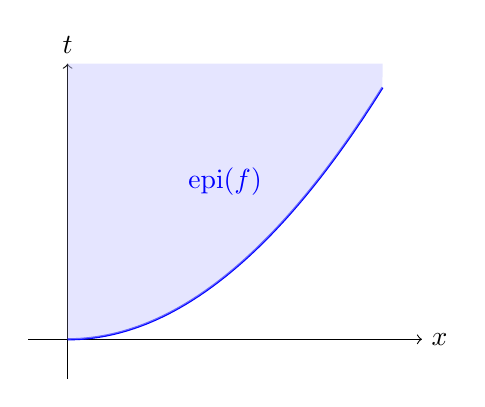
\begin{tikzpicture}
    % Axes
    \draw[->] (-0.5,0) -- (4.5,0) node[right] {$x$};
    \draw[->] (0,-0.5) -- (0,3.5) node[above] {$t$};
    
    % Convex function
    \draw[thick, blue] plot [domain=0:4, samples=100] (\x, {0.2*\x*\x});
    
    % Epigraph
    \fill[blue!20, opacity=0.5] (0,0) -- plot [domain=0:4, samples=100] (\x, {0.2*\x*\x}) -- (4,3.5) -- (0,3.5) -- cycle;
    
    % Label
    \node[blue] at (2,2) {epi$(f)$};
  \end{tikzpicture}
  \caption{Epigrafen til en konveks funksjon}
  \label{fig:epigraph}
\end{figure}

\subsection{Dualitet i Konveks Optimering}
\begin{definition}{Lagrangian-Dualitet}{lagrangian_duality}
  For det konvekse optimeringsproblem
    \begin{mini}
      {x}{f(x)}{}{}
      \addConstraint{g_i(x)}{\leq 0,}{i = 1,\ldots,m}
      \addConstraint{Ax}{= b}{}
    \end{mini}
  er Lagrangian-funksjonen $\mathcal{L}(x,\lambda,\nu) = f(x) + \sum_{i=1}^m \lambda_i g_i(x) + \nu^T(Ax-b)$ hvor $\lambda_i \geq 0$. 
  Dualfunksjonen er $g(\lambda,\nu) = \inf_x L(x,\lambda,\nu)$ og dualproblemet er
    \begin{maxi}
      {\lambda,\nu}{g(\lambda,\nu)}{}{}
      \addConstraint{\lambda}{\geq 0}{}
    \end{maxi}
\end{definition}

\begin{theorem}{Sterk Dualitet}{strong_duality}
  Hvis et konvekst optimeringsproblem tilfredsstiller Slaters betingelse (dvs. det eksisterer et strengt mulig punkt), da gjelder sterk dualitet: de optimale verdiene av primal- og dualproblemet er like.
\end{theorem}

\section{Konveksitet - Sammendrag}
% First table: Basic Concepts
\begin{table}[H]
  \centering
  \begin{tabular}{|p{3cm}|p{5cm}|p{6cm}|}
    \hline
    \rowcolor{blue!25}
    \textbf{Konsept} & \textbf{Definisjon} & \textbf{Matematisk Formulering} \\
    \hline
    Konveks Mengde & En mengde hvor ethvert linjesegment mellom to punkter i mengden ligger helt i mengden &
    \(C\subset \mathbb{R}^n\) er konveks hvis:
    \[\forall x,y\in C,\;\alpha\in [0,1]:\] 
    \[\alpha x + (1-\alpha) y\in C\] \\
    \hline
    \rowcolor{blue!5}
    Konveks Funksjon & En funksjon hvor grafen ligger under linjesegmentet mellom to punkter på grafen &
    \(f: C \to \mathbb{R}\) er konveks hvis:
    \[f(\alpha x + (1-\alpha) y)\;\le\]\[\alpha f(x) + (1-\alpha) f(y)\] 
    for alle \(x,y\in C,\;\alpha\in [0,1]\) \\
    \hline
  \end{tabular}
  \caption{Grunnleggende konsepter innen konveksitet}
  \label{tab:basic_concepts}
\end{table}

% Second table: Characterizations
\begin{table}[H]
  \centering
  \begin{tabular}{|p{3cm}|p{5cm}|p{6cm}|}
    \hline
    \rowcolor{rem-color!25}
    \multicolumn{3}{|l|}{\textbf{Karakteriseringer av Konveksitet}} \\
    \hline
    \rowcolor{rem-color!5}
    1. Ord. Bet. & Tangentapproks. ved ethvert punkt er en global underestimator &
    For deriverbar \(f\), konveksitet er ekvivalent med:
    \[f(y)\;\ge\; f(x) + \nabla f(x)^\mathsf{T} (y - x)\]
    \[\forall x,y \in C\] \\
    \hline
    2. Ord. Bet. & \(H_f(x)\) er pos. semidefinit overalt i \(C\) &
    For \(f \in C^2\), konveksitet er ekvivalent med:
    \[\nabla^2 f(x) \succeq 0\quad \forall x \in C\] \\
    \hline
  \end{tabular}
  \caption{Karakteriseringer av konveksitet}
  \label{tab:characterizations}
\end{table}

% Third table: Important Results
\begin{table}[H]
  \centering
  \begin{tabular}{|p{3cm}|p{5cm}|p{6cm}|}
    \hline
    \rowcolor{cor-color!25}
    \multicolumn{3}{|l|}{\textbf{Viktige Resultater}} \\
    \hline
    \rowcolor{cor-color!5}
    Jensens Ulikhet & Funksjonsverdien av et vektet gjennomsnitt er mindre enn \newline
    eller lik det vektede gjennomsnittet av funksjonsverdiene &
    For konveks \(f\) og vekter \(\alpha_i \geq 0\) med \(\sum_i \alpha_i = 1\):
    \[f\Bigl(\sum_i \alpha_i x_i\Bigr)\;\le\;\sum_i \alpha_i f(x_i)\] \\
    \hline
    Epigraf & Mengden av alle punkter som ligger på eller over grafen til funksjonen &
    \(\mathrm{epi}(f)=\{(x,t) \mid x\in\mathrm{dom}(f), t\ge f(x)\}\)
    
    \(f\) er konveks \(\Leftrightarrow\) \(\mathrm{epi}(f)\) er konveks \\
    \hline
    \rowcolor{cor-color!5}
    Subgradient & Generalisering av gradient for ikke-deriverbare funksjoner &
    En vektor \(g\) er en subgradient av konveks \(f\) ved \(x\) hvis:
    \[f(y)\;\ge\; f(x) + g^\mathsf{T}(y-x)\quad \forall y \in C\] \\
    \hline
  \end{tabular}
  \caption{Viktige resultater innen konveksitet}
  \label{tab:important_results}
\end{table}

% Fourth table: Optimization Theory
\begin{table}[H]
  \centering
  \begin{tabular}{|p{3cm}|p{5cm}|p{6cm}|}
    \hline
    \rowcolor{prop-color!25}
    \multicolumn{3}{|l|}{\textbf{Optimeringsteori}} \\
    \hline
    \rowcolor{prop-color!5}
    Lokale/Globale\newline Minima & For konvekse problemer er\newline ethvert lokalt minimum\newline også et globalt minimum & 
    For konveks \(f\) på konveks \(C\):\newline\quad\(\text{lokal min} \iff \text{global min}\) \\
    \hline
    Sterk Dualitet & Under visse betingelser er det ingen dualitetsgap &
    Under Slaters betingelse: 
    \[\text{primal opt.} = \text{dual opt.}\] \\
    \hline
  \end{tabular}
  \caption{Optimeringsteori og konveksitet}
  \label{tab:optimization_theory}
\end{table}


\section{Betydning i Optimering}
Konveksitet er avgjørende i optimering av flere viktige grunner:

\begin{itemize}
    \item \textbf{Global Optimalitet}: Konvekse optimeringsproblemer har et unikt globalt minimum hvis streng konveksitet holder, siden ethvert lokalt minimum er globalt.
    
    \item \textbf{Forenklede Optimalitetsbetingelser}: Førsteordens optimalitetsbetingelser er tilstrekkelige for global optimalitet, noe som forenkler analyse og løsningsmetoder.
    
    \item \textbf{Algoritmisk Effektivitet}: Det finnes effektive algoritmer for å løse konvekse optimeringsproblemer, inkludert gradientmetoder, indrepunktsmetoder og proksimalmetoder.
    
    \item \textbf{Praktiske Anvendelser}: Mange praktiske problemer innen maskinlæring, kontrollteori, signalbehandling og finans kan formuleres som konvekse optimeringsproblemer eller tilnærmes av dem.
    
    \item \textbf{Dualitetsteori}: Konveksitet muliggjør kraftige dualitetsresultater som gir alternative løsningsmetoder og sensitivitetsanalyse.
\end{itemize}


\paragraph{Oppsummering av Konveksitet}
Konvekse mengder og funksjoner spiller en sentral rolle i optimering fordi de gir problemer som er relativt enkle å analysere og (ofte) mye enklere å løse, både teoretisk og algoritmisk. 
Den viktige egenskapen om at \emph{lokale minima er globale} gjør det mulig å forenkle beregningene betydelig og gir sterke konvergensegenskaper for standardalgoritmer som gradientmetoder, indrepunktsmetoder, subgradientmetoder, og så videre.
